\section{Calibration Cost Accounting}

Figure~\ref{fig:calibration-cost-vs-quality} visualizes the same cost rows as
Table~\ref{tab:calibration-cost-summary}. The x-axis is logarithmic because the
matched prompt batches are small relative to the per-guidance calibration
cost. Positive quality values favor ours; negative values favor the base
schedule under the reported metric.

\begin{figure}[t]
  \centering
  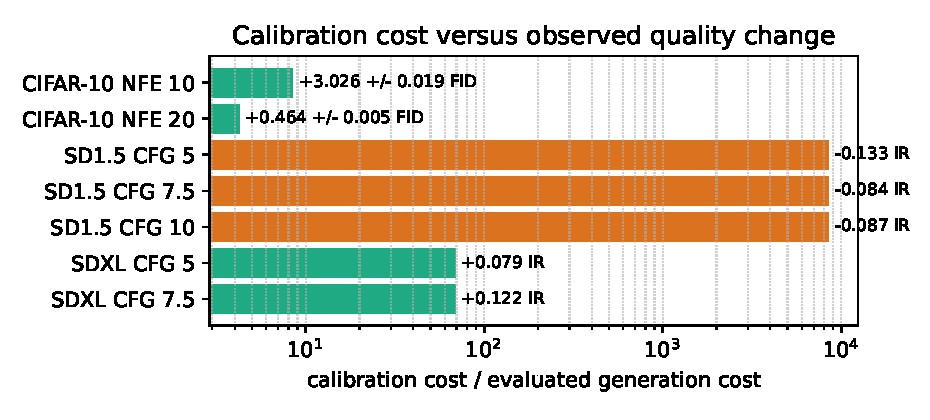
\includegraphics[width=0.9\linewidth]{figures/calibration_cost_vs_quality.pdf}
  \caption{Calibration cost versus observed quality change for current
  paper-facing runs. CIFAR-10 uses base-minus-ours FID, so positive values
  mean lower FID for ours. Text-to-image rows use ours-minus-base ImageReward,
  so negative values mean lower ImageReward for ours. Model-evaluation
  equivalents count retained calibration cost divided by the evaluated
  generation batch cost.}
  \label{fig:calibration-cost-vs-quality}
\end{figure}

The source CSV, table, and figure are generated by the aggregation script under
\texttt{paper/figures/src/}. The cleaned summary is stored under
\texttt{paper/results/cost/}.

\begin{table}[t]
  \centering
  \caption{Calibration amortization under reuse of the same schedule.
  Columns report calibration overhead divided by generation cost after
  reusing the schedule for $M$ evaluated-size batches. Break-even is the
  smallest integer $M$ for which calibration cost is no larger than
  generation cost.}
  \label{tab:calibration-amortization-summary}
  \small
  \begin{tabular}{lllrrrr}
    \toprule
    Setting & condition & quality vs. base & $M=1$ & $M=10$ & $M=100$ & break-even \\
    \midrule
    CIFAR-10 & NFE 10 & +3.026 $\pm$ 0.019 FID & 8.49$\times$ & 0.85$\times$ & 0.08$\times$ & 9 \\
    CIFAR-10 & NFE 20 & +0.464 $\pm$ 0.005 FID & 4.24$\times$ & 0.42$\times$ & 0.04$\times$ & 5 \\
    SD1.5 & CFG 5 & -0.133 IR & 8{,}487$\times$ & 848.70$\times$ & 84.87$\times$ & 8487 \\
    SD1.5 & CFG 7.5 & -0.084 IR & 8{,}487$\times$ & 848.70$\times$ & 84.87$\times$ & 8487 \\
    SD1.5 & CFG 10 & -0.087 IR & 8{,}487$\times$ & 848.70$\times$ & 84.87$\times$ & 8487 \\
    SDXL & CFG 5 & +0.079 IR & 68.62$\times$ & 6.86$\times$ & 0.69$\times$ & 69 \\
    SDXL & CFG 7.5 & +0.122 IR & 68.62$\times$ & 6.86$\times$ & 0.69$\times$ & 69 \\
    \bottomrule
  \end{tabular}
\end{table}


Table~\ref{tab:calibration-amortization-summary} shows that the current CIFAR
runs need schedule reuse across several evaluated-size batches before
calibration overhead falls below generation cost. The actual CIFAR reuse check
in Table~\ref{tab:cifar10-pndm-euler-50k-reuse-seed0-schedule} supports this
amortization only for the retained PNDM/CIFAR Euler execution grid. The SD1.5
sweep would require thousands of matched prompt batches to amortize the
calibration cost, and its observed ImageReward deltas are negative. The SDXL
sweep uses a lighter calibration setting and breaks even after 69 matched
prompt batches, but this arithmetic still needs positive reused-schedule
quality before deployment efficiency becomes supported.
